\documentclass[12pt,letterpaper]{article}
%%%%%%%%%%%%%%%%%%%%%%%%%%%%%%
%Force pdflatex processing even with "$ latex" (required by arXiv)
\pdfoutput=1
%%%%%%%%%%%%%%%%%%%%%%%%%%%%%

\usepackage[utf8]{inputenc}
\usepackage{amsmath}
\usepackage{amssymb}
\usepackage{amsthm}
\usepackage{fp}
\usepackage{xcolor}
\definecolor{nicered}{rgb}{0.7,0.1,0.1}
\definecolor{nicegreen}{rgb}{0.1,0.5,0.1}
\usepackage[colorlinks=true,citecolor= nicegreen,linkcolor=nicered]{hyperref}
\usepackage{graphicx}
\usepackage[separate-uncertainty=true]{siunitx} 
\usepackage{cancel}

\setlength{\textwidth}{180mm}
\setlength{\oddsidemargin}{-1cm}
\setlength{\evensidemargin}{-1cm}
\setlength{\topmargin}{-1cm}

\title{Dark matter}

\author{Notes from Course by Enrico Nardi\\ LNF-INFN}
\begin{document}
\maketitle

\section{Introduction}

\section{PReamble}
$1/\gamma\sim$ time scale of a reaction.

In an effective theory of early universe the high temperature can render some of the parameters zero, and the symmetries are increased. For example, of $T\gg m$, the mass terms become irrelevant.


\section{General relativity}
Radiation dominated $p=\rho/3$
\begin{align*}
  \dot\rho=&-4\rho\frac{\dot{a}}{a}\nonumber\\
  \frac{d\rho}{\rho}=&-4\frac{da}{a}
\end{align*}
and
\begin{align*}
  \rho\sim a(t)^{-4}\,.
\end{align*}

Matter dominated: $p=0$
\begin{align*}
  \dot{\rho}=&-3\rho\frac{\dot{a}}{a}\nonumber\\
  \frac{d\rho}{\rho}=&-3\frac{da}{a}
\end{align*}
and
\begin{align*}
  \rho\sim a(t)^{-3}\,.
\end{align*}

Critical density
\begin{align*}
  \rho_c=\frac{3H^2}{8\pi G}
\end{align*}
Something useful is
\begin{align*}
  h=\frac{H}{\SI{100}{Km/s/Mpc}}
\end{align*}
where $h=0.7$ and $h^2=1/2$.

If  $ \rho\sim a(t)^{-4}$

\begin{align*}
  H=&\sqrt{\frac{8\pi G}{3}\rho}\nonumber\\
&=\sqrt{\frac{8\pi G}{3}}a^{-2}
\end{align*}

and from
\begin{align*}
  \frac{d\rho}{dt}=-4\rho H
\end{align*}


we obtain
\begin{align*}
  t\sim \frac{1}{2}\sqrt{\frac{3\rho}{8\pi G}}=\frac{1}{2}H^{-1}\,.
\end{align*}
In natural units
\begin{align*}
  \gamma_X\sim H
\end{align*}
\begin{align*}
  f(\mathbf{p})=
  \left(
   e^{(E-\mu)/T\pm 1}|_{-B}^{+f}
  \right)
\end{align*}
\begin{align*}
  n=\frac{g}{2\pi^3}\int f(\mathbf{p})d^3p
\end{align*}
\begin{align*}
  \rho=\frac{g}{2\pi^3}\int E(\mathbf{p}) f(\mathbf{p})d^3p
\end{align*}
\begin{align*}
  P=\frac{g}{2\pi^3}\int \frac{\mathbf{p}^2}{3E} f(\mathbf{p})d^3p
\end{align*}

In the non-relativistic approximation
\begin{align*} 
n=
\left(
\frac{mT}{2\pi}
\right)^{3/2} e^{(m-n)/T}
\end{align*}
\begin{align*}
  \rho=mn
\end{align*}
\begin{align*}
  P\sim T\cdot n\sim 0
\end{align*}

\begin{align*}
   H=&\sqrt{\frac{8\pi G}{3}\rho_\text{rad}}\nonumber\\
&=\sqrt{\frac{8\pi G}{3}}a^{-2}
\end{align*}
where
\begin{align*}
  \rho\approx \frac{\pi^2}{30}g_* T^4
\end{align*}
where
\begin{align*}
  G=1/M_p^2
\end{align*}
Therefore
\begin{align*}
  H=&\sqrt{\frac{8\pi\pi^2}{3\cdot 30}}\sqrt{g_*}\frac{T^2}{M_p}\nonumber\\
=& 1.66\sqrt{g_*}\frac{T^2}{M_p}\nonumber\\
=&17\cdot \frac{T^2}{M_p}\,.
\end{align*}

\subsection{Degrees of fredom}


\begin{itemize}
\item[Quarks:] $(6\times 2\times2)\times 3=72$
\item[Gluons:] $8\times 2=16$
\item[Leptons:] $3\times 2\times2=12$
\item[Neutrinos:] $3\times 2=6$
\item[$H_0$:] $1$
\item[$\gamma$:] $2$
\item[$W^{\pm},Z$:] $3\times3=9$
\end{itemize}

\begin{align}
  \rho_{\text{rad}}=\frac{\pi^2}{30}T^4
  \left[
\sum_b g_b
\left(
\frac{T_b}{T}
\right)^4
\frac{7}{8}\sum_f g_f
\left(
\frac{T_b}{T}
\right)^4
  \right]
\end{align}
and
\begin{align}
   \rho_{\text{rad}}=\frac{\pi^2}{30}g_* T^4\,,
\end{align}
where
\begin{align}
  g_*=&(16+12)+\frac{7}{8}(90)\nonumber\\
 =&301
\end{align}

\subsection*{Example}
\begin{align}
  p+\bar{\nu}&\longleftrightarrow n+e^+\nonumber\\
  p+e&\longleftrightarrow n+\nu\nonumber\\
\end{align}
\begin{align}
  \sigma\sim G_F^2 T^2 M_p \sim\SI{1.2E19}{GeV}?
\end{align}
\begin{align}
  n_\nu\sim  T^3
\end{align}
\begin{align}
  n_\nu\sigma\sim G_F^2 T^5\longleftrightarrow 1.66\sqrt{g_*}
\frac{T^2}{M_p}\sim H
\end{align}

\section{Freeze-out of $N-\bar{N}$ annihilation}
\begin{itemize}
\item $\sigma_A\sim (1/m_{\pi})^2\sim (\SI{1}{fm})^2$
\item $T_{\text{f.o}}?$
\end{itemize}
\begin{align}
  T_{\text{f.o}}>&m_N\sim \SI{1}{GeV} & n\sigma &\longleftrightarrow 1.66\sqrt{g_{*}}\frac{T^2}{M_p}\nonumber\\
&&  T^3 \frac{1}{m_{\pi}^2}& \longleftrightarrow 10 \frac{T^2}{M_p}
\end{align}

\begin{align}
  g_{*}(T<\SI{100}{MeV}):& 3\nu+\gamma+e^{\pm}\nonumber\\
&\frac{7}{8}(3\cdot 2+4)+2=\frac{43}{4}
\end{align}
\begin{align}
   g_{*}(\SI{100}{MeV}<T<\SI{1}{GeV}):& \mu,\pi,k,\omega,\rho,k^{*}\nonumber\\
     %falta
    &=\frac{55}{2}
\end{align}

\begin{align}
  (n_{f})^{\text{rec}}\sim& \frac{3}{4}\frac{\zeta(3)}{\pi^2}g T^3&
T& \longleftrightarrow 10m_{\pi}\left( \frac{m_{\pi}}{m_p} \right)
\end{align}

\begin{align}
  (n_f)\sim& g \left( \frac{m_N T}{2\pi} \right)e^{-m/T} & x=m/T \nonumber\\
 \sim& \left( \frac{g}{(2\pi)^{3/2}} \right) T^3 x^{3/2}e^{-x}=1.7\times 3.3 \frac{T^{2}}{M_{p}}m_{\pi}
\end{align}
further details (two lines) until
\begin{align}
  \frac{1}{2}\log x-x=-20\times 2.3
\end{align}
\begin{align}
  x_{\text{f.o}}=\frac{m_N}{T_{\text{f.o}}}\sim 48
\end{align}
\begin{align}
  T_{\text{f.o}}=\frac{m_N}{48}\sim \SI{21}{MeV}
\end{align}
\begin{align}
  \frac{n_N^{(\text{relic})}}{n_{\gamma}}\sim \frac{1}{4}(48)^{3/2}e^{-48}
  \frac{T^3}{T^3}\sim 10^{-19}
\end{align}

\begin{align}
  \eta_{b}\equiv \frac{n_B-n_{\bar{B}}}{n_{\gamma}}=(5.7\pm 0.6)\times 10^{-10}
\end{align}


Consider the process $e^+e^-\to \mu^+\mu^-$ mediated by a photon, with a cross section proportional to $\alpha^2/s$, or
\begin{align}
  \sigma\sim \alpha^2/T^2\,.
\end{align}
For the same process but mediated by $Z$, with $T\ll  M_Z$
\begin{align}
  \sigma_Z\sim G_F^2 E^2\sim G_FT^2 
\end{align}
Note that the last expression contains also the first one in the limit $T\gg M_Z$.

\emph{missing plot in function of $1/T$}

For example, for $T\gg \Lambda_{\text{GUT}}$, then all the reactions
\begin{align*}
  T^3\sigma\sim \frac{\alpha^2}{T^2}T^3\sim \alpha^2T\Leftrightarrow 17\cdot \frac{T^2}{M_P}
\end{align*}
\begin{align*}
  T\sim 10^{-4}\cdot \SI{10E19}{GeV}
\end{align*}
clearly outside of equilibrium

\section{Dark Matter}

\subsubsection{Cold relics}

Cold relics make the freeze-out in the non-relativistic regime or
$T_{\text{f.o}}\ll m_X$, where $X$ is the particle itself. But in
cosmology means that the particles in non-relativist at
matter/radiation equality. Remember that $\rho_{\text{rad}}\sim T^{4}$
and $\rho_{\text{mat}}\sim T^{4}$. Therefore, after some time the
matter will be dominating.  This is the beginning of the structure
formation epoch. This structure formation is only possible if there is
the required dark matter is cold or warm.  Note that the two
freeze-out definitions are different.


According to the first definition we need to use one Boltzmann
suppressed distribution.
\begin{align*}
  n_x\sim& T^3 x^{3/2}e^{-x}\nonumber\\
  \sigma_x\times \left( T^3x^{3/2}e^{-x} \right)\sim
  \frac{T^2}{M_p}\sim \left( \frac{m_x^2}{M_P} x^{-2} \right)
\end{align*}
where
\begin{align*}
  x=\frac{m_X}{T}
\end{align*}
Therefore
\begin{align*}
  \sigma_x \left( \frac{T}{m}x^{3/2} e^{-x} \right)\sim \frac{1}{M_P m_x}
\end{align*}
\begin{align*}
  x^{1/2}e^{-x}\sim \frac{1}{M_P m_x \sigma_x}
\end{align*}
For a typical cross section
%%missing
\begin{align*}
  \sigma_x\sim G_F^2 m_x^2\sim \left( 10^{-5} \text{GeV}^{-2}
  \right)^2\cdot \left( \SI{10E2}{GeV} \right)^2\,,
\end{align*}
\begin{align*}
  x^{1/2}e^{-x}\sim \frac{1}{10^{18} 10^{2} 10^{-8}}\sim 10^{-13}
\end{align*}
and,
\begin{align*}
  x_{\text{f.o}}=13\times 2.3\sim 30
\end{align*}
If instead of $10^{-13}$ we use the range $10^{-10}-10^{-20}$
\begin{align*}
  x_{\text{f.o}}\sim 20-50\,.
\end{align*}
The freeze-out is determined from the initial number of particles and
the cross section. It is assumed that the initial number of particles
is produced termically.

The distribution density over $T^3$ as a function of  $x$ we have the
plot of fig.~\ref{fig:1}.


\subsubsection{Relic density}

\begin{align}
\label{eq:Om}
  \Omega_{x}=&\frac{m_x n_x^0}{\rho_c}
\end{align}
where $n_x^0$ is the density number today. Moreover, as
\begin{align*}
  na^3=&n_0 a_0^3 \nonumber\\
 n_0=& n_{\text{f.o}}\frac{a^3}{a_0^3}=n_{\text{f.o}}\left( \frac{T_0}{T_{\text{f.o}}} \right)^3
\end{align*}
and replacing back in (\ref{eq:Om})
\begin{align}
  \Omega_x=&\frac{m_x}{\rho}n_{\text{f.o}}\frac{T_0^3}{T_{\text{f.o}}}
 =\frac{T_0}{\rho_c}x_{\text{f.o}}\left(
   \frac{m_{\text{f.o}}}{T_{\text{f.o}}} \right)^3 \nonumber\\
=& \frac{T_0^3}{\rho_c}x_{\text{f.o}}\frac{1}{M_P \sigma_x}
\end{align}
\begin{align}
  n_{\text{f.o}}\sigma=\frac{T_{\text{f.o}}^2}{M_P}
\end{align}


Some numbers
\begin{align}
  \rho_c=1.05\times10^{-5}h^2 \text{GeV\ cm}^{-3}=10^{-47}h^2\text{GeV}^4
\end{align}
Then we have
\begin{align*}
T_0=&\SI{2.7}{K}\nonumber\\
 k=&\SI{8.6E-5}{eV K}^{-1}=1 \nonumber\\
\SI{1}{K}=&\SI{8.6E-5}{eV}
\end{align*}
Therefore
\begin{align*}
  \Omega_x=&\frac{T_{\text{f.o}}^3}{\rho_c}\times 20 \frac{1}{M_P}\frac{1}{\sigma_x}\nonumber\\
=&\frac{10^{-38}}{10^{-47}}20 \frac{1}{10^{19}}\frac{1}{\sigma_x}\left( \frac{x_{\text{f.o}}}{20} \right)\nonumber\\
=&10^{-9}\frac{1}{\sigma_x}\left( \frac{x_{\text{f.o}}}{20}
\right)\times {2}
\end{align*}
Normalizando al valor experimental del $20\%$
\begin{align*}
  \frac{\Omega_{x}}{0.2}=10^{-8}\frac{1}{\sigma_x}\left( \frac{x_{\text{f.o}}}{20}\right)
\end{align*}
The typical cross-section is
\begin{align*}
  \sigma_{\text{EW}}\sim &G_F^2 T_{\text{f.o}}^2 \nonumber\\
                   \sim &G_F^2 \frac{m_x^2}{(20)^2} \nonumber\\
\sim & 10^{-10}\times \frac{1}{4} 10^2 \times 10^{2}\times 10^{2}\nonumber\\
 \sim& 0.25\times 10^{-6}\sim \SI{2.5E-9}{GeV}^{-2}
\end{align*}
to be compared with the typical cross section of
\begin{align*}
  \sigma_x\sim \SI{1E-8}{GeV}^{-2}\,.
\end{align*}

However the relevant quantity is the thermal average
\begin{align*}
  \left\langle \sigma v \right\rangle
\end{align*}
which for $x=m_x/T_{\text{f.o}}\sim 20\sim \frac{m}{\frac{1}{2}m
  v^2}$ $\to v^2\sim 1/10$ and $v\sim 1/3$ instead of $1$ for a
relativistic particle. 

Therefore
\begin{align*}
  [\sigma]\sim& \text{cm}^{2}\nonumber\\
  [v]\sim&\text{cm/s}
\end{align*}
and
\begin{align*}
   \left\langle \sigma v \right\rangle\sim \SI{1E-8}{GeV}^{-2}\left(
     \SI{2E-14}{GeV cm} \right)^2\times \frac{1}{3}3\times\SI{1E10}{cm/s}
\end{align*}
\begin{align*}
   \left\langle \sigma v \right\rangle\sim \SI{3E26}{cm^3/s}
\end{align*}
This suggest indirect signals of dark matter. It the dark halo of our
Galaxy is used to know the local density of Dark Matter, it is
possible to prove the cross section of the center of Galaxy with the
current satellite experiments.

\subsubsection{Cold relics}
Some facts
\begin{itemize}
\item $m_x\sigma M_P\gg 1$
\item $\sigma \sim \SI{1E-8}{GeV}$
\end{itemize}
\begin{align}
  \sigma\sim g^4/m_I
\end{align}
for some particle intermediate $I$. 
\begin{align}
  \frac{g^2}{m_I}&\sim \SI{1E-4}{GeV}\to & g^2&\sim \frac{m_I}{\SI{1}{TeV}}
\end{align}
with
\begin{align}
  M_p\gg \frac{1}{m_x\sigma }\sim \frac{\SI{1E8}{GeV}^2}{m_x}
\end{align}
and
\begin{align}
  m_x\gg \frac{\SI{1E8}{GeV}^2}{M_P}\sim \SI{1E-11}{eV}\sim \SI{1E-2}{eV}
\end{align}


\begin{figure}
  \centering
  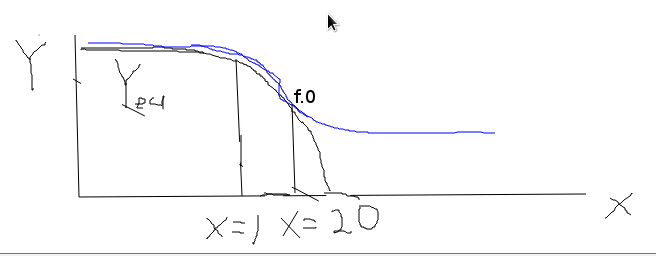
\includegraphics[scale=0.5]{fig2}

  \caption{Figure}
  \label{fig:1}
\end{figure}


%\bibliographystyle{h-physrev4}%apsrev4-1long
%\bibliography{susy}


\end{document}

%%% Local Variables: 
%%% mode: latex
%%% TeX-master: "dm"
%%% End: 